%--------------------------------------------------------%
%	TITLE
%--------------------------------------------------------%

\chapter[Domestic Well Vulnerability to Drought Duration and Unsustainable Groundwater Management in California's Central Valley.]{Domestic Well Vulnerability to Drought Duration and Unsustainable Groundwater Management in California's Central Valley.\footnote[1]{This chapter has been published: Pauloo, R. A., Escriva-Bou, A., Dahlke, H., Fencl, A., Guillon, H., \& Fogg, G. E. (2020). ``Domestic well vulnerability to drought duration and unsustainable groundwater management in California’s Central Valley''. \textit{Environmental Research Letters}, 15(4), 044010.}}


%--------------------------------------------------------%
%	ABSTRACT
%--------------------------------------------------------%

\section{Abstract}
    
\noindent Millions of Californians access drinking water via domestic wells, which are vulnerable to drought and unsustainable groundwater management. Groundwater overdraft and the possibility of longer drought duration under climate change threatens domestic well reliability, yet we lack tools to assess the impact of such events. Here, we leverage 943,469 well completion reports and 20 years of groundwater elevation data to develop a spatially-explicit domestic well failure model covering California's Central Valley. Our model successfully reproduces the spatial distribution of observed domestic well failures during the severe 2012-2016 drought (n = 2,027). Next, the impact of longer drought duration (5 to 8 years) on domestic well failure is evaluated, indicating that if the 2012-2016 drought would have continued into a 6- to 8-year long drought, a total of 4,037 - 5,460 to 6,538- 8,056 wells would fail. The same drought duration scenarios with an intervening wet winter in 2017 lead to an average of 498 and 738 fewer well failures. Additionally, we map vulnerable wells at high failure risk and find that they align with clusters of predicted well failures. Lastly, we evaluate how the timing and implementation of different projected groundwater management regimes impact groundwater levels and thus domestic well failure. When historic overdraft persists until 2040, domestic well failures range from 5,966 - 10,466 (depending on the historic period considered). When sustainability is achieved progressively between 2020 and 2040, well failures range from 3,677 - 6,943, and from 1,516 - 2,513 when groundwater is not allowed to decline after 2020. 


%--------------------------------------------------------%
% Introduction
%--------------------------------------------------------%
\section{Introduction}

Presently, more than 13 million households rely on private domestic wells for drinking water in the United States \citep{uscensus2017}. In the State of California alone, around 1.5 million residents rely on domestic wells for drinking water, around one third of which live in the Central Valley (CV) \citep{Dieter2018}. Domestic wells in the CV are greater in number than agricultural or public supply wells, yet tend to be more shallow and have much smaller pumping capacities (e.g., 0.25 - 1.0 $m^3/hr$ compared to 100.0 - 900.0 $m^3/hr$ \citep{Harter2003}). Well completion report data \citep{oswcr} suggest that between 1900 and 2018 in the CV, 96,299 domestic wells with an interquartile (IQR) depth range of 36.6 - 75.6 $m$ were drilled, compared to 43,861 agricultural wells (IQR: 57.9 - 152.0 $m$) and 3,649 public supply wells (IQR: 76.2 - 159.0 $m$). Hence, a large number of shallow domestic wells in the CV are vulnerable to both lowering of the groundwater table \citep{theis1935relation, theis1940source, sophocleous2000safe, Greene2018, Perrone2019} and contamination by pollutants such as total dissolved solids \citep{Cismowski2006, Bertoldi1991}, nitrates \citep{Harter2012, Balazs2011, Ransom2017}, arsenic \citep{Welch2000, Ahuja2008}, uranium \citep{Jurgens2008, Fujii1995}, and hexavalent chromium \citep{Robertson1991, Ellis2002}, among others. 

Past droughts in California have encouraged both additional well drilling and groundwater pumping to supplement dwindling surface water supplies \citep{Hanak2011, Medellin-azuara2016}. During the 2012-2016 drought, 2,027 private domestic drinking water wells were reported dry in California's CV \citep{observedDW}; because reporting was voluntary, actual well failure counts are possibly greater. To date, limited long-term data and solutions exist to address the vulnerability of rural community drinking water supply wells to severe droughts \citep{Mitchell2017, Feinstein2017}. 

The paucity of well failure research, particularly in California, is partially due to privately-held records on well location and construction. In 2017, the public release of over one hundred years of digitized domestic Well Completion Reports (WCR) enabled the first spatial distribution and count estimates of domestic wells in California \citep{Johnson2015, Johnson2017}. The California Online State Well Completion Report Database (OSCWR) \citep{oswcr} and similar well construction databases across the U.S. have allowed near-continental scale estimation of failing wells \citep{Perrone2017} and well depths \citep{Perrone2019}. A recent study in the Tulare County, California (around 5,000 $km^2$) estimated domestic well supply interruptions from groundwater level decline during the 2012-2016 drought, and the associated costs of maintaining domestic water well supplies \citep{Gailey2019}. However, to our knowledge, no studies have developed models at the regional aquifer scale (around 50,000 $km^2$ or greater) that simulate the impact of drought and sustainable groundwater management regimes on domestic well failure. Such a model can help evaluate the consequences of future droughts and statewide groundwater management options. 

Groundwater overdraft in California is part of a larger global trend in aquifer depletion \citep{Famiglietti2014, wada2010global, doll2012impact, siebert2010groundwater}. Like many other semi-arid, agriculturally intensive regions worldwide, in the decades to come, California will grapple with the impacts of climate change and policy on its overdrafted aquifers. By the end of the 21st century, California's snowpack is projected to decline by as much as 79.3\% \citep{Rhoades2018}, and drought frequency in the southern CV may increase by upwards of 100\% \citep{Swain2018}. It is in this increasingly drier and warmer climate \citep{Diffenbaugh2015, Cook2015} characterized by more frequent, more spatially extensive heat waves and extended droughts \citep{Tebaldi2006, Lobell2011}, that California will implement a statewide policy of sustainable groundwater management \citep{SGMA}. These policies aim to prevent chronic groundwater overdraft and other undesirable results, including domestic well failure. However, we lack both methodological approaches to forecasting well failure, and a basic understanding of how climate change (i.e., drought) and policy (i.e., groundwater management regimes) will impact well failure.  

In this paper, we present a regional aquifer scale model covering California's CV that predicts domestic well failure in response to groundwater level decline from extended drought and different groundwater management regimes. The model was developed using reported domestic well failures from the severe 2012-2016 California drought. The goal of this study is to evaluate the risk of domestic well failure in response to 1) extended (5 to 8 year) drought duration scenarios and 2) three different groundwater management regimes (sustainability, glide path, business as usual) in California's CV.   


%--------------------------------------------------------%
% Study Area
%--------------------------------------------------------%
\section{Study area}

The domestic well failure model was developed for the California CV alluvial groundwater basin (Figure \ref{fig:study_site}). We chose this area for its geologic continuity, data availability, social and economic significance, and high rates of domestic well failure reported during the recent 2012-2016 drought. The study area was further pared down to only include areas with domestic wells completed on or after 1976 (SI Appendix \ref{ap_a_study_area}).  

% 16_study_site_figs.R
% code/00_figures/study_site/pnas_study_site3.ai
\begin{figure}%[tbhp]
	\centering
	\includegraphics[width=\textwidth]{ch2_figs/fig_study_site3.pdf}
	\caption{California's Central Valley is a major agricultural hub in the Western US, approximately 720 $km$ long and 64 to 97 $km$ wide. (A) The 2,027 reported domestic well failures during the 2012-2016 drought (red dots) cluster in the southeast. 67,011 domestic wells (blue dots) reported in OSWCR and constructed after 1976 were used to define the study area (SI Appendix \ref{ap_a_study_area} for details). (B) Average groundwater level change from 2012-2016 in unconfined to semi-confined aquifers. Areas of large groundwater level decline correspond to areas of high reported well failure.}
	\label{fig:study_site}
\end{figure}

The CV is heavily dependent on winter snowpack and groundwater for agriculture \citep{Scanlon2012, Faunted.2009, Hanak2011}. 
In an average year, groundwater provides about 30\% of the water demand, but in drought years, groundwater can account for upwards of 60\% of water consumed in some parts of the CV \citep{Brush2013}. Nearly all of this water is consumed by agriculture \citep{Brush2013, Faunted.2009}. 
It is well established that scarce surface water supply during drought encourages groundwater pumping \citep{Lund2018, Feinstein2017, Mount2018}. The United States Geologic Survey estimated that during periods of drought, groundwater pumping in the CV increased upwards of 180\% compared to the long-term mean (1962-2003) \citep{Faunted.2009}. 
Estimated annual baseline groundwater depletion in the San Joaquin Valley (southern CV) is 2.3 $km^3/yr$, but during drought, the groundwater depletion rate may be up to 5 times greater \citep{Hanak2019}. 
Modeled CV groundwater depletion during the 1976-1977, 1987-1992, 2012-2016 droughts is estimated at 24.6 $km^3$, 49.3 $km^3$, and 40.0 $\pm$ 0.8 $km^3$ respectively \citep{Scanlon2012, Xiao2017}.
Thus, four- and five-year long historical droughts in California's CV have led to groundwater storage losses roughly equivalent to the combined storage capacity of California's surface water reservoirs (51.8 $km^3$) \citep{Hanak2011}.  

Groundwater storage change leads to groundwater level change. Data from 506 monitoring wells in the Tulare Lake hydrologic region indicate that between fall 2011 and fall 2017, around 90 \% of wells experienced a decline in groundwater level, and 58.9 \% of wells experienced more than 7.5 $m$ of groundwater level decline \citep{dwrgwl2017}. 



%--------------------------------------------------------%
% Methods
%--------------------------------------------------------%
%%%%%%%%%%%%%%%%%%% Data
\subsection{Data}
The study used well completion reports from 943,469 wells from the California Department of Water Resources (\hyperlink{https://data.ca.gov/dataset/well-completion-reports}{data.ca.gov/dataset/well-completion-reports}) \citep{oswcr}. Further, the study used seasonal groundwater level measurements \citep{gwl} spanning the period 1998-2017 and well failures reported during the 2012-2016 drought. The well failure dataset was obtained via an agreement with the California Department of Water Resources and the California Governor's Office of Planning and Research \citep{observedDW}. A limitation of the reported well failure data is that data was neither collected nor verified consistently by counties, and reporting was voluntary (and usually happens only when a well owner could not self-solve their issues). Hence, the reported data under-counts the domestic wells impacted during the drought. All data are accessible online \citep{Pauloo2019}, with the exception of observed well failure data, which are confidential and may be obtained by contacting the California Department of Water Resources. Further information on data sources is provided in SI Appendix \ref{ap_a_data}.

%%%%%%%%%%%%%%%%%%% Conceptual model of well failure
\subsection{Classification of failing and vulnerable wells}

We distinguish between three classes of well status: \textit{active}, \textit{failing}, and \textit{vulnerable}. A well is classified as \textit{active} when the groundwater level at the location of the well is above the level of the pump intake. If the groundwater level falls at or below the pump intake, the well is classified as \textit{failing} (Figure \ref{fig:conceptual_model_wf}). The well failure data collected during the 2012-2016 drought did not distinguish between failing wells and wells experiencing a decrease in pump efficiency, thus for the model calibration, wells are considered as either failing or active. Further detail is provided in SI Appendix \ref{ap_a_formal_wf}.

Wells are classified as \textit{vulnerable} to well failure when the groundwater level in a well falls within 3 $m$ of the pump intake. As the distance between a well's pump intake and the groundwater level decreases, the fluid pressure (i.e. the net positive suction head) declines, causing cavitation, which may physically damage the pump and decrease its efficiency \citep{Tullis1989, Helweg1983}. In this study, we estimate the minimum separation distance required to avoid decreases in well function as 3 $m$ (see SI Appendix \ref{ap_a_vi}).
%Vulnerability is mapped in the four extended drought scenarios discussed in \ref{ss_2_7}, and in one additional scenario close to present day groundwater levels at the time of writing (Fall 2018).  

% code/00_figures/conceptual_mod/pnas_conceptual_mod.ai
\begin{figure}%[tbhp]
	\centering
	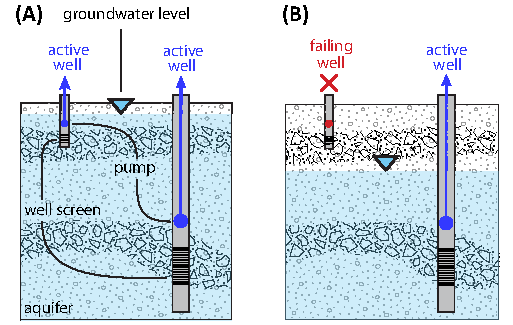
\includegraphics[width=\textwidth]{ch2_figs/fig_conceptual_mod.pdf}
	\caption{Conceptual model of well failure in an unconfined to semi-confined alluvial aquifer (details provided in SI Appendix, \ref{ap_a_formal_wf}). (A) Groundwater level is above all pump intakes, and all wells are active. (B) Groundwater level falls below the pump intake of the shallow well, causing it to fail. The deep well remains active. In our study site, shallow wells tend to be domestic, and deep wells tend to be agricultural and public supply wells.}
	\label{fig:conceptual_model_wf}
\end{figure}


%%%%%%%%%%%%%%%%%%% GW level interpolation
\subsection{Groundwater level interpolation}

Seasonal (spring and fall) groundwater level data for each year between 1998 and 2017 \citep{gwl} were used to determine groundwater level changes in the unconfined to semi-confined shallow aquifer, which domestic wells draw from. For each set of seasonal groundwater levels, we applied ordinary kriging to the log-transformed groundwater levels to normalize the data distribution, suppress outliers, and improve data stationarity \citep{DeutschC.V.andJournel1992, Varouchakis2012}. Because the expected value of back-transformed log-normal kriging estimates is biased (i.e. not equal to the sample mean), we applied the correction of Laurent \citep{Laurent1963, JournelA.G.Huijbregts1978} to recover unbiased groundwater level estimates (SI Appendix \ref{ap_a_gwl}). We further calculated the 5\% and 95\% confidence intervals of the kriging estimates to propagate kriging uncertainty through the model and into the well failure estimates.   


%%%%%%%%%%%%%%%%%%% Pump depth imputation
\subsection{Pump intake depth estimation}

Pump intake depth is not explicitly recorded on WCRs, thus for each well, it was estimated as the mean of the static water level at the time of well completion, and the top of the screened interval (SI Appendix \ref{ap_a_pump_depth}). When pump depth could not be directly calculated (i.e. - a WCRs is missing static water level or the top of the screened interval information), we imputed pump depths with simple linear models to regress known pump depths onto the bottom of the screened interval, which is known for nearly all wells (SI Appendix Figure \ref{fig:pump_loc_bottom}). Pump depth exhibits spatial variance due to geologic heterogeneity and historical groundwater level, hence imputation was conducted at the Bulletin 118 subbasin level (SI Appendix Figure \ref{fig:pump_loc_density}) to ensure hydrogeologic similarity. As with the kriging estimates, we calculated the 5 and 95\% confidence intervals of the estimated pump locations to propagate this uncertainty into the well failure estimates.    

%%%%%%%%%%%%%%%%%%% Calibration
\subsection{Model calibration based on 2012-2016 drought data}

The well failure model was calibrated with observed 2012-2016 well failures by relating groundwater level changes to estimated pump intake locations of wells in OSWCR, and minimizing error between the observed and predicted well failures during the 2012-2016 drought (SI Appendix \ref{ap_a_calib}). Well failures tend to form clusters, thus we calculated Gaussian kernel density estimates for the observed and predicted point patterns and calculated residual error as their difference. We use a kernel bandwidth of 433 $m$, calculated as $0.15 / \sqrt{5 \cdot \lambda}$ where $\lambda$ is the point intensity--the number of observations divided by the study site area \citep{stoyan1994fractals}. Calibration results are depicted at the Public Land Survey System \citep{us2009manual} township resolution (roughly 10 $km$) to improve mapping.




%%%%%%%%%%%%%%%%%%% drought duration scenarios
\subsection{Simulation of drought duration scenarios}

Climate change may cause severe and extended droughts exceeding 4 years in duration, yet the impact of such drought durations on domestic well failure remains unknown. Thus, we simulate drought durations of 5 to 8 years in length by extending the observed 2012-2016 drought with an additional 1 to 4 years using two scenarios:  

\begin{enumerate}
	\item \textit{Continuous drought}: 1 to 4 years of drought immediately following the 2012-2016 drought.
	\item \textit{Intervening wet winter}: identical to the continuous drought scenario, but groundwater levels are allowed to recover after 4 years, due to one intervening wet winter. 
\end{enumerate}

Groundwater level change in each drought duration scenario was determined by assuming that the impact of future droughts is proportional to the historical 2012-2016 drought. In other words, the groundwater level change associated with 1 to 4 additional years of drought is computed by scaling the change in the groundwater level field observed during the 2012-2016 drought by 0.25, 0.50, 0.75, and 1 respectively. 

In the ``continuous drought'' scenario, groundwater levels are already low from the 2012-2016 drought, and increased well failure is expected. Hence, the ``intervening wet winter'' scenario examines how much a wet winter event, such as the one observed in 2017, may buffer against well failure over a longer drought duration.  



%%%%%%%%%%%%%%%%%%% GW management regimes
\subsection{Projected groundwater management regimes}

In California, the Sustainable Groundwater Management Act (SGMA) enacted in 2014, requires the development and implementation of local groundwater management plans by 2020. These plans aim to prevent undesirable results, including the chronic lowering of groundwater levels, to achieve groundwater sustainability by 2040 for critically overdrafted basins.
%, and by 2042 for the remaining high and medium priority basins. 
Overlying landowners of overdrafted basins may deploy different groundwater management regimes, which will impact groundwater level change in the coming decades to various degrees.  

To analyze how different groundwater management regimes might impact groundwater level change and hence domestic well failure, we simulate three simplified regimes for the period 2017 -- 2040 (Figure \ref{fig:SGMAscenarios}): 

\begin{enumerate}
	\item \textit{Strict sustainability}: water levels do not decline after 2020. This represents a theoretical (and idealized) best case management regime for domestic wells.  
	\item \textit{Glide path}: groundwater level decline is gradually reduced over the implementation period until 2040.  
	\item \textit{Business as usual}: groundwater level decline continues at the historic rate. This regime is used for comparison.  
\end{enumerate}


% code/00_figures/alvar_scens
% .R and .ai files: pnas_sgma.ai
\begin{figure}%[tbhp]
	\centering
	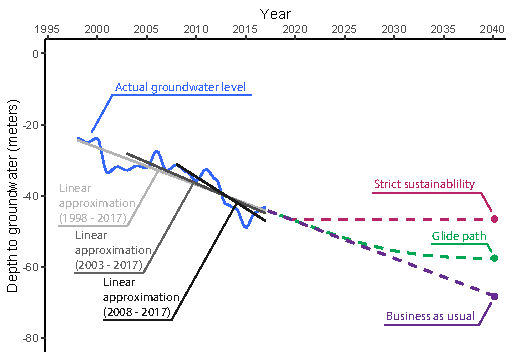
\includegraphics[width=\textwidth]{ch2_figs/fig_sgma.pdf}
	\caption{Projected groundwater management regimes using actual groundwater elevation change for a point in Tulare County as an example. Groundwater level change is approximated by three linear trends, based on different time periods. In this figure, we show the different projected groundwater management regimes using the linear approximation based on the 1998-2017 period. In the analysis, we calculate groundwater levels across the entire CV, using all three trends, and all three regimes.}
	\label{fig:SGMAscenarios}
\end{figure}

To project the number of failing wells for each groundwater management regime, we extend past groundwater level trends through 2040. For this, we first determined past groundwater level trends using data for the period from 1998-2017 and estimated annual groundwater levels at each point of the CV via ordinary kriging as discussed above and in SI Appendix section \ref{ap_a_gwl}. To estimate declining groundwater level trends consistently over time, we only use fall measurements following the growing season. We then obtain linear approximations of groundwater level for each cell using a 5x5 $km^2$ raster. We use three different approximations of groundwater level based on changes observed from 1998-2017, 2003-2017, and 2008-2017 to account for differences in initial groundwater level and thus, uncertainty introduced by the period over which the linear models are built. Finally, to project the ``Strict sustainability'' regime we extend these three approximations into 2020, then eliminate further overdraft. In contrast, the ``Business as usual'' regime projects the linear trends into 2040 before ending overdraft, and the ``Glide path'' regime gradually reduces the slope of the linear trend between 2020 to 2040, representing a middle path between the ``Strict sustainability'' and the ``Business as usual'' regimes. 




%--------------------------------------------------------%
% Results
%--------------------------------------------------------%
\section{Results}

\subsection{Well failure prediction during the 2012-2016 drought}

The calibrated model reproduced both the magnitude and spatial distribution of the 2,027 well failures observed in the study area during the 2012-2016 drought (Figure \ref{fig:pred_obs}A). The model predicts a slightly higher mean number of well failures (n = 2,513) (Figure \ref{fig:pred_obs}B), which is expected, as observed well failures are most probably under-reported due to the voluntary nature of data collection, and a well-owner's perceived consequence of reporting a failed well to their county or state. 

The normally distributed residual error (Figure \ref{fig:pred_obs}C) indicates the unbiasedness and strength of the model: well failure predictions for the observed 2012-2016 drought were within 20\% of the actual value for around 68.2\% of the study area, between 20\% and 55\% of the actual value for around 27.2\% of the study area, and greater than 55\% of the actual value for less than 5\% of the study area. 

Unsurprisingly, both observed and predicted failures tend to cluster in the southeastern CV, where agricultural groundwater use is comparatively higher than elsewhere in the state \citep{Brush2013, Faunted.2009}; households reliant on domestic wells in this region are particularly susceptible to failure. 


% 07_spatial_density_obs_and_pred.Rmd
% code/00_figures/pred_obs/pnas_pred_obs_accuracy.ai
\begin{figure}%[tbhp]
	\centering
	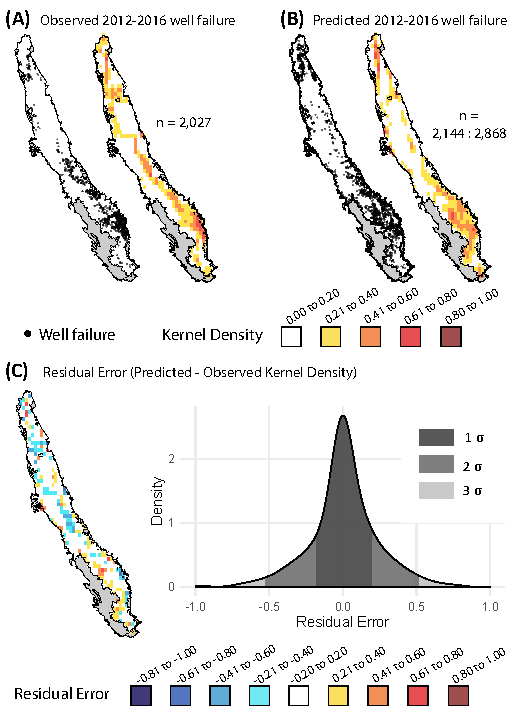
\includegraphics[width=12cm,keepaspectratio]{ch2_figs/fig_pred_obs_accuracy.pdf}
	\caption{Model performance in predicting the spatial intensity of observed domestic well failures during the 2012-2016 drought. (A) Observed well failure point pattern and kernel density estimate. (B) Predicted well failure mean estimate (n = 2,513) and kernel density of the mean prediction. The 5 and 95\% confidence intervals of predicted well failures span the interval from 2,144 - 2,868. (C) Residual (predicted minus observed) error. Red areas indicate areas of over-prediction, and blue areas indicate under-prediction.}
	\label{fig:pred_obs}
\end{figure}



%%%%%%%%%%%%%%%%%%% Drought duration scenarios
\subsection{Failing and vulnerable wells in drought duration scenarios}

Longer drought duration results in widespread well failure episodes concentrated primarily in the southeastern CV (Figure \ref{fig:p_1_2_3_4}). Consistent with domestic well failure patterns observed during the 2012-2016 drought, well failure density is highest in Madera, Kings, Kaweah, Tule, Tulare Lake, and Kern subbasins.  

% pred_1_2_3_4 in `09_plot_pred_future_failures.Rmd`
% density_pred_1_2_3_4 in `09_plot_pred_future_failures.Rmd`
% code/00_figures\pred_1_2_3_4/pnas_pred_1234_small_2.ai
\begin{figure}%[tbhp]
	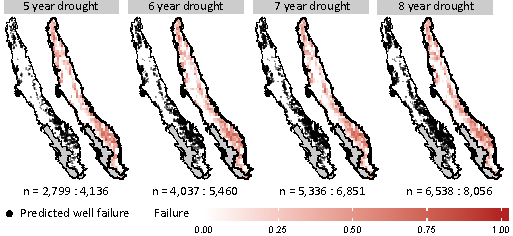
\includegraphics[width=\textwidth]{ch2_figs/fig_pred_1234_small_2.pdf}
	\caption{Simulated domestic well failure point patterns and associated kernel density estimates for 5 to 8 year drought duration scenarios beginning in Fall 2016 (maps show mean prediction). $n$ is the 5 and 95\% confidence interval of cumulative well failure count in each scenario, including the 2,027 failing wells in the 2012-2016 drought.}
	\label{fig:p_1_2_3_4}
\end{figure}

In the ``continuous drought'' simulation, two- and four-year long droughts immediately following the 2012-2016 drought (6 and 8 years total without an intervening wet winter) result in 4,037 to 5,460 and 6,538 to 8,056 cumulative well failures, respectively. Thus, a two-year drought duration following the 2012-2016 drought results in more well failures than the 2012-2016 drought alone, and a combined 8 year drought duration results in nearly twice the failures observed from 2012-2016 (Figure \ref{fig:cum_sum_failure}). Intensified well failure during extended drought reinforces the interdependence of well failure on groundwater level: when groundwater levels cannot recover to pre-drought levels and pump depths are fixed, wells are more vulnerable to failure.  

% `cum_sum_failures.pdf` in figures/code
% `p` in `13_trendline_d-2012_2016_and_future_d.Rmd`
% code/00_figures/cum_sum_fail/pnas_cum_sum_fail.ai
\begin{figure}%[tbhp]
	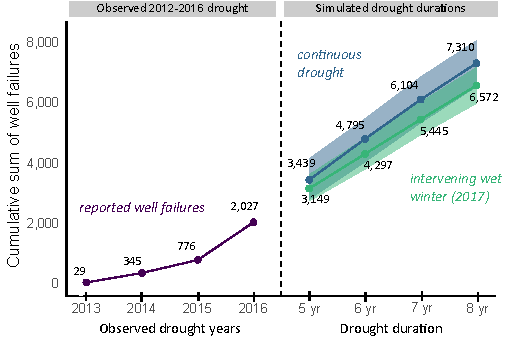
\includegraphics[width=\textwidth]{ch2_figs/fig_cum_sum_fail.pdf}
	\caption{Left: Cumulative domestic well failures from 2012-2016. Right: Cumulative domestic well failures resulting from simulated drought durations 5 to 8 years in length. The continuous drought duration scenario (blue) leads to more well failure compared to the intervening wet winter scenario (green). Points represent the mean well failure estimate, and shaded regions represent the 5 and 95\% confidence intervals. %Observed well failures from 2012-2016 reflect when the failure was reported, not necessarily when the well actually failed. Data collection by the state did not begin in a systematic way until late 2014, and many of the reports received in 2016 may be motivated by the fact that the state made financial assistance available to households on private wells in this year.
	}
	\label{fig:cum_sum_failure}
\end{figure}


In the ``intervening wet winter'' scenario, groundwater levels are allowed to recover during 2017, and well failure slightly abates: 498 and 738 fewer wells fail in the 6 and 8 year drought scenarios, indicating that an increase in median groundwater level of only a few meters across the Central Valley can prevent hundreds of domestic well failures during extended drought.  

%The cumulative sum of annual well failures observed during the 2012-2016 drought follows an exponential trend; in simulated extended drought scenarios, it follows a linear trend (Figure \ref{fig:cum_sum_failure}). If the drought were to continue past the simulated 8 years scenario, well failures would follow a sigmoidal trend: inflecting then leveling off, as failure progresses to increasingly infrequent and deeper wells until none are left.  

The cumulative sum of annual well failures observed in the evaluated drought duration scenarios follows a linear trend (Figure \ref{fig:cum_sum_failure}). If the drought were to continue past the simulated 8 years scenario, well failures likely would follow a sigmoidal trend: inflecting then leveling off, as failure progresses to increasingly infrequent and deeper wells until none are left.  

Vulnerable wells (Figure \ref{fig:vi}) are those with estimated pump intakes within 3 $m$ of the groundwater level, and are at heightened risk of experiencing a reduction in pump efficiency, or a failure episode. Since this 3 $m$ window is fixed in our analysis, the spatial distribution and count of vulnerable wells is relatively constant across the drought duration scenarios (2,274 to 2,453 wells), and the present day scenario of Fall 2018 (mean estimate = 2,568). Moreover, the spatial distribution of vulnerable wells mirrors those of well failures.

% figure starts in code/15_vulnerability_index.R
% 00_figures/vi/pnas_vi.ai 
\begin{figure}
	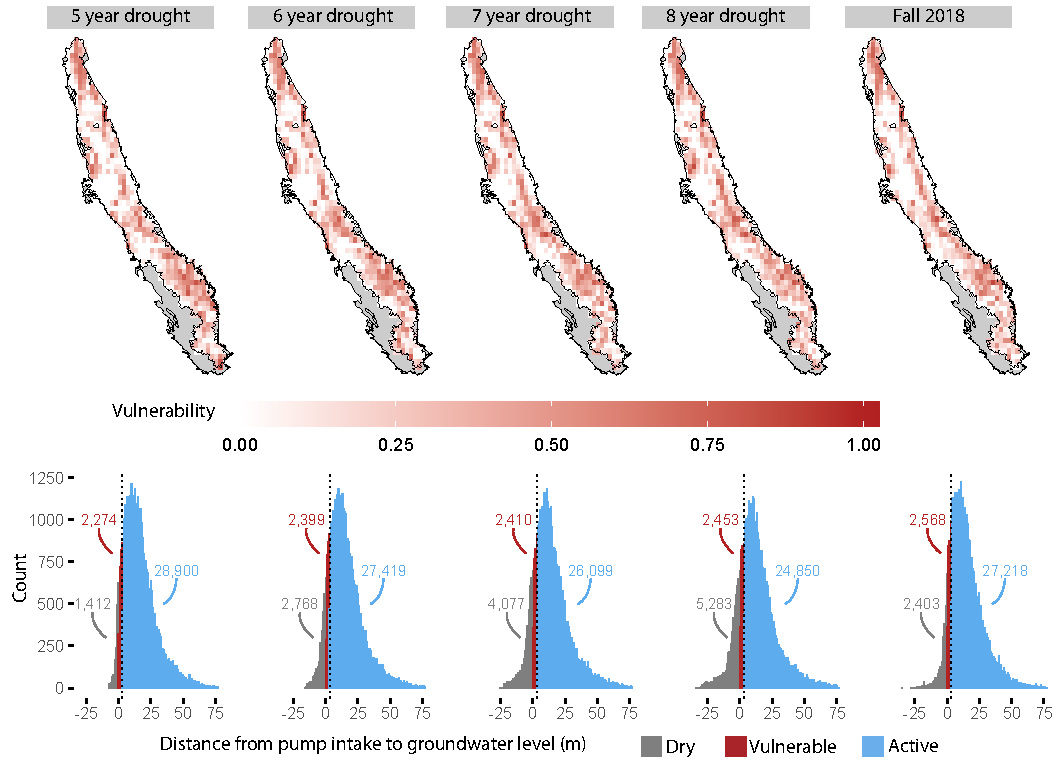
\includegraphics[width=\textwidth]{ch2_figs/fig_vi.pdf}
	\caption{Top row: kernel density estimates of low vulnerability (white) and high vulnerability (red) regions in extended drought duration scenarios and in Fall 2018. Bottom row: histograms of failing wells (grey), vulnerable wells (red), and active wells (blue) for the extended drought scenarios and Fall 2018 scenario. The black dotted line at 3 meters is the threshold at which wells are at risk of decreased efficiency. All numbers reported are the mean estimate of dry, vulnerable, and failing wells.}
	\label{fig:vi}
\end{figure}



%%%%%%%%%%%%%%%%%%% sustainable management regimes
\subsection{Failing wells in projected groundwater management regimes}

Projecting groundwater depths into 2040 under three different management regimes results in significant differences in domestic well failures (Figure \ref{fig:sgma_grid}). The ``Business as usual'' regime, with no change in the historical trend of groundwater level decline, would lower the groundwater level by up to 100 $m$ in parts of the southern CV, but significant groundwater level declines are widespread. Scenarios aimed at achieving sustainability would reduce these declines, hence the differences between the ambitious ``Strict sustainability'', ``Glide path'' and ``Business as usual'' pathways might be quite important for water resources managers and policy makers.

The groundwater depth changes and associated well failures are sensitive to the period used for the linear approximation of groundwater level declines. The period from 2008-2017 leads to significantly worse groundwater depletion than both periods 2003-2017 and 1998-2017, particularly because of the effects of the 2012-2016 drought. Average well failures for the ``Business as usual'' regime range from 5,966 to 10,466 (depending on the period used for the linear interpolation), while under the ``Glide Path'' regime they range from 3,677 to 6,943, and from 1,516 to 2,513 under the ``Strict sustainability'' regime (confidence intervals are reported in SI Appendix Table \ref{tab:dom_failures}).  

% 18_run_model_2.R for simulation and plotting. paths below outdated.
% 00_figures/alvar_scens/pnas_sgma_grid_trim.ai
% 12_sustainable_gw_mgnt_scenarios.Rmd for:
% pnas_sgma_gwl_change.pdf | pnas_sgma_gwl_change_grid.pdf
% pnas_sgma_dry_wells.pdf | pnas_dry_well_grid.pdf
% 00_figures/alvar_sgma/sgma_scens.R for pnas_sgma_trends.pdf
\begin{figure}
	\includegraphics[width=\textwidth]{ch2_figs/fig_sgma_grid_trim.pdf}
	\caption{Domestic well failures projected for three groundwater management regimes (columns) based on three different time periods of linear groundwater level change (rows). The left plot of each pair is the mean projected groundwater level change from 2017-2040. Groundwater level decline (red) is more common than groundwater level increase (blue). The right plot of each pair shows the mean predicted well failure point pattern for that combination of groundwater management regime and groundwater level change approximation. See SI Appendix Table \ref{tab:dom_failures} for confidence intervals.}
	\label{fig:sgma_grid}
\end{figure}
%TC:endignore
\clearpage

Most of the estimated domestic well failures are still concentrated in the southeastern CV, but the central and northern CV are also affected, presumably due to the ubiquity of relatively shallow wells in these regions. The ``Business as usual'' regime leads to especially severe well failure in all three projected groundwater level trends.



%--------------------------------------------------------%
% Discussion
%--------------------------------------------------------%
\section{Discussion}


%%%%%%%%%%%%%%%%%%% 
\subsection{Impact of drought duration on well failure and vulnerability}

It is well understood that drought duration leads to increased groundwater extraction \citep{Hanak2011, Medellin-azuara2016}, and hence domestic well failure \citep{Perrone2017, Feinstein2017}. Thus, we tested the impact of previously unseen drought durations ranging 5 to 8 years in length, by simulating an additional 2 to 4 years of severe drought immediately following the 2012-2016 drought, calculating the change in groundwater level, and determining failing and vulnerable wells. 

%Unlike existing regional-scale analyses \citep{Perrone2017}, the domestic well failure model developed in this study improves upon existing well failure models in terms of spatial scale \citep{Gailey2019}, and allows for scenario testing. 
A previous study estimated that 4 years of drought in the Tulare County, California immediately following the 2017 wet winter would result in about 200 - 850 domestic well failures \citep{Gailey2019}. 
Our model's equivalent scenario (intervening wet winter with an 8 year drought duration) results in a similar range of 585 - 715 domestic well failures in Tulare County. Additional comparisons are not possible given the lack of research on this topic.  

At the level of California's CV, our results suggest that drought durations of 6 to 8 years result in 4,037 to 5,460 and 6,538 to 8,056 cumulative well failures, respectively. However, an intervening wet winter during the 6- and 8-year long drought duration simulations buffers against well failure: when groundwater is allowed to recover after 4 years of drought (as happened during the 2017 wet winter), an average of 498 and 738 less domestic wells fail. These findings support research indicating that limiting groundwater pumping during drought may reduce well failure \citep{Hanak2019, Gailey2019}, and a general understanding that groundwater pumping can lower proximal groundwater levels \citep{theis1935relation}.  

During the 2012-2016 drought, the median groundwater level in the CV fell to progressively new historic lows each fall after the summer growing season (SI Appendix \ref{ap_a_drought_impact}) \citep{dwrgwl2017}. Our results indicate that between fall of 2014 and 2015, the median groundwater level across the entire CV fell by nearly 5 $m$, and in some areas (i.e. - Tulare, Kings, and Kern counties), by tens of meters. In fall of 2016, the median groundwater level in the CV was 27.0 $m$ below land surface. Moreover, our results indicate that the interquartile range of domestic well pump locations in the CV is 24.5 to 52.3 $m$ below land surface. The proximity of pump intake depths to groundwater levels explains why domestic wells are sensitive to even slight declines in groundwater level: 5 to 10 $m$ of groundwater level decline may easily impact thousands of domestic well pump intakes and cause failure. 

In the four drought duration scenarios evaluated, an average of 2,274 to 2,453 domestic well pumps reside within 3 $m$ of the groundwater level. We classified these wells as vulnerable, because they are likely to fail first under persistent groundwater level decline. The spatial distribution of well vulnerability mirrors that of well failures. Mapping clusters of predicted failing and vulnerable wells is essential for sustainable water management and disaster response.


%%%%%%%%%%%%%%%%%%% 
\subsection{Implications for groundwater management and policy}

The strong dependence of domestic well failure on groundwater pumping to support irrigated agriculture raises serious questions concerning the role of sustainable groundwater policy in mitigating well failure \citep{Hanak2019}. We evaluated three different projected groundwater management regimes to curb groundwater level declines in the coming years: a ``Strict sustainability'' theoretical best-case regime wherein declining trends in groundwater level stop in 2020, a ``Business as usual'' regime that continues groundwater decline until 2040, and a final ``Glide path'' moderate regime that slows the rate of groundwater level decline to the midway point between the former two regimes.  

Our results suggest that choices embedded within each of the groundwater management regimes vastly impact the amount of expected well failures. For instance, the ``Glide path'' regime predicts 3,677 to 6,943 domestic well failures by 2040, and the ``Business as usual'' regime predicts 5,966 to 10,466 domestic well failures by 2040. Both groundwater management regimes would result in twice to almost three times as many well failures than the ``Strict Sustainability'' regime (1,516 to 2,513 failures). All three scenarios are sensitive to the period of record used to approximate the linear groundwater level decline, however they underpin the vulnerability of domestic wells to historic rates of groundwater level decline, and demonstrate the impact of management on well failure.  

Refilling overdrafted aquifers via managed aquifer recharge might meet the dual objectives of increasing groundwater storage, and bolstering domestic well dependent households' drought resilience. In California, high-magnitude flood flows are likely the most accessible and largest sources of water to replenish groundwater aquifers through managed aquifer recharge \citep{Kocis2017}, which might considerably slow or reverse trends in groundwater depletion. The emerging research in the strategic siting of managed aquifer recharge considers impacts on crop health \citep{Dahlke2018}, human health \citep{ayuso2011quantifying}, the mobilization of contaminants into groundwater \citep{Xanke2017}, and hydrogeologic suitability (i.e. - highly conductive flowpaths and geologic formations capable of accommodating large volumes of water, such as incised valley fills) \citep{Maples2019}. In the San Joaquin Valley where domestic well failures peak, managed aquifer recharge alone may not be enough to offset groundwater overdraft, but coupled with a reduction in agricultural water use \citep{Hanak2019}, groundwater levels may stabilize enough to prevent widespread future failure events. 

This study assumes that no interim well construction takes place to prepare for falling groundwater levels, such as the practice of pump lowering or well deepening. Pump lowering typically takes place in 6 $m$ intervals (the length of standard discharge piping), and costs around \$2,000 USD per lowering event \citep{Gailey2019}. If we consider the cost of pump lowering in all failing wells in the 6- and 8-year drought duration scenarios (in reality some wells will not have room to be lowered) and assuming every failing well's pump is lowered once (some will require more than one lowering), at \$2,000 USD per 6 $m$ unit of discharge piping, 4,037 - 5,460 and 6,538- 8,056 failures correspond to \$8.7 - \$10.4 and \$13.8 - \$15.5 million USD. 

During the recent drought, it is likely that some households also deepened their wells. In California and nationwide, drilling deeper wells is a common practice to adapt to declining groundwater levels \citep{Perrone2019}, but is a costly and unsustainable solution that may furthermore result in cross-contamination due to interconnection of confined aquifers by well construction \citep{gailey2017inactive}. Moreover, the financial burden of pump lowering or well deepening might disproportionately impact disadvantaged populations \citep{Famiglietti2014} unable to afford chasing after declining groundwater levels. Since many of these disadvantaged groups may not own their land and thus wells, well construction decisions may be made by landowners rather than the affected groups.  

%%Underpinning the dilemma of domestic well failure is the urgent need for an adequate cost estimation to facilitate sensible short- and long-term policy solutions. 
Sustainable long-term solutions for drinking water access might include connecting vulnerable households to nearby centralized water provisions. Recent research indicates that many rural communities, assumed to be on domestic wells, are actually quite close (less than 2 $km$) to a potable water supply system \citep{London2018}. However, as annexation and consolidation is financially and physically impractical for all domestic-well dependent households, many will remain too remote and isolated to connect to a nearby water system.  

%We currently lack a thorough understanding of the economic burden of well failure and how it may affect demographic groups disproportionately. 
Short- and long-term solutions to domestic well failure remain largely unexplored. What role can managed aquifer recharge play in mitigating well failure? Given the strong dependence of groundwater level decline on extraction for irrigated agriculture, could agri-business proximal to centers of high well failure collectively fund safety nets that internalize the cost of well failure during periods of increased groundwater pumping? Should vulnerable domestic well reliant populations connect to nearby municipal water systems with more reliable water supply? What is the appropriate solution for those that are too remote or isolated to connect to a community system? 

%%%%%%%%%%%%%%%%%%% 
\subsection{Applicability to other areas}

The well failure model presented in this study is extensible to other areas outside of California where sufficient data or groundwater flow models are available. It relies on two inputs: (1) a time series of spatially-explicit groundwater level surfaces reflecting typical groundwater level changes (specifically, the maximum drawdown), and (2) well construction information (i.e. - geographic location and pump intake depth). 

Approaches for interpolating groundwater levels and estimating pump intake depths are demonstrated in this study, though others exist \citep{Gailey2019, Perrone2017, OSullivan2010, JournelA.G.Huijbregts1978}. Groundwater levels provided by a groundwater flow model such as MODFLOW \citep{Harbaugh2000} would easily couple to a well failure model, enabling the simulation of water management regimes and the impact of the resulting groundwater level on domestic well failure at arbitrary temporal scales. In California, existing regional-scale groundwater flow models such as C2VSim \citep{Brush2013} and CVHM \citep{Faunted.2009} can be used to plan for the impact of future failure episodes under different water management regimes involving changes in both pumping and recharge in space and time. 

This study aimed for regional prediction of failing, vulnerable, and active wells, but more nuanced impact analyses can be made. For instance, variable losses in well efficiency may be quantified as groundwater levels fall \citep{Medellin-azuara2016}. This in turn enables the cost estimation of repairing failing and vulnerable wells (e.g. - pump lowering, well deepening), compared to water management actions (e.g. - fallowing fields, reduced groundwater pumping).  

Where resources exist to survey households, detailed domestic well information such as geographic location, pump intake depth, and retirement age may be obtained, and would further constrain the uncertainty inherent in the estimation of these parameters. Additionally, well failure observations are essential for model calibration. Though this study benefited from failure data, efforts to anticipate domestic well failures as proactive hazard mitigation should not wait for the existence of observational data. It does, however, suggest the benefit of having such a system in place as part of local and state-level drought preparedness.  

%%%%%%%%%%%%%%%%%%% 
\subsection{Implications for adaptation to climate change}

Our results demonstrate that the mechanisms leading to domestic well failure are heavily dependent on groundwater level declines due to pumping for irrigated agriculture and increased pumping during drought. A historical lack of groundwater management in California \citep{Hanak2011} has led to widespread groundwater level decline. Climate change compounds the impact of water management decision-making. Warming will increase the frequency and duration of drought in California and other parts of the world \citep{Diffenbaugh2015, Cook2015, Swain2018, Rhoades2018, VanLoon2016}, and if left unchecked, groundwater withdrawal will likely intensify as surface water becomes more scarce, as it has in the past \citep{Hanak2011}. As we demonstrate in this study, groundwater replacement of lost surface water during extended drought intensifies well failure due to already low groundwater levels. Thus, managing for low to no domestic well failure requires a consideration of the complex interaction between land use change, water resources management, human decision-making, and climate change. Unless adaptation strategies become integral to sustainable groundwater management policy, the extended droughts anticipated under climate change and resulting changes in groundwater levels will put thousands of domestic wells in California's CV at risk of failure, and hence, thousands of Californians at risk of losing access to water.  


%%%%%%%%%%%%%%%%%%% 
\subsection{Additional perspective on the data and model}

%% This study is one example of how state-led initiatives towards open data, or the practice of releasing previously-private databases to the public, enables research towards previously inaccessible questions. This study benefited from open data tabulated in a machine-readable format, which simply would not have been possible otherwise. By comparison, while former studies have dedicated many hours to statistically sample and manually read nearly three quarters of a million WCRs \citep{Johnson2015}, we were able to automate the reading and QAQC process for nearly one million tabulated WCRs. This reinforces existing and nascent efforts to transition data-collection and storage to standardized, digital, and machine-readable formats that can be easily accessed and manipulated by scientific scripting languages.  

There is generally good agreement between the observed and predicted well failure at the 10 $km$ resolution of the residual error maps (Figure \ref{fig:pred_obs}A-B), and better agreement (Figure \ref{fig:pred_obs}C) is achieved at larger spatial scales (i.e. - Bulletin 118 groundwater subbasins, entire CV). Thus, the results presented in this study should not be taken as \textit{de facto} predictions of the exact locations of well failure, but rather, as \textit{regional-scale} well failure estimates. Local-scale errors introduced by uncertainty in well failure reporting, well completion reporting, groundwater level, and model formulation are overcome at regional scales. 

We acknowledge that spatial and temporal variability in monitoring well data introduces uncertainty in the interpolated groundwater level. Ambient monitoring wells measured each season (i.e. - spring and fall) are not the same across seasons, and each season's measurements are sampled over a roughly three month time frame (January-March in the spring, and October-December in the fall). However, because most of the groundwater level change observed in a year takes place as the result of the summer growing season, and the fall measurements take place after the summer, spring and fall measurements still reflect ambient conditions. Moreover, both scaling the 2012-2016 groundwater level change to create future drought scenarios, and calculating 2040 groundwater levels with linear trends are simple approaches to estimate future groundwater level decline, but the accuracy of any method to forecast unseen future events are also questionable. Additionally, we do not account for any emergency response measures in response to drought such as groundwater pumping curtailments. In California, some households were able to drill deeper wells, lower their pumps, or connect to a nearby surface water supply system during the drought. Because these corrective actions are cost-prohibitive and highly unlikely to be widespread, our modeling assumptions (no corrective action) and hence results, still agree with observed well failure rates from 2012-2016. 




%--------------------------------------------------------%
% Conclusion
%--------------------------------------------------------%
\section{Conclusions}

%% More than one million Californians rely on private domestic wells for drinking water, and nearly half a million of these people live in the CV. Owing to their relatively shallow depth, domestic wells often fail first when groundwater levels fall, as observed during the 2012-2016 drought. As water resource managers aim to stabilize groundwater level declines, climate warming threatens to increase drought frequency and duration in California. We currently lack drought preparedness tools for regional-scale estimation of domestic well failure, and the ability to rapidly assess future well failure under different groundwater level scenarios. 

In this study, we developed a data-driven well failure model and applied it to California's CV to make regional-scale estimates of domestic well failure, and assess future well failure under different groundwater level scenarios.  

Our model reproduces reported domestic well failures during the 2012-2016 drought in California's CV ($n$ = 2,027), and furthermore, simulates the impact of different drought duration scenarios up to 8 years in length. We show that small declines in groundwater level are sufficient to cause thousands of wells failures when groundwater levels are already low, and that wet winters, and hence groundwater recharge or reduced pumping, may buffer against well failure. A simulated drought duration of 6 years (2012-2018) results in 4,037 - 5,460 total well failures. Similarly, an 8-year long drought (2012-2020), corresponds to a median groundwater level change of less than 10 $m$ across the CV, but results in 6,538- 8,056 total well failures. The same 6 and 8 year long drought duration scenarios with an intervening wet winter in 2017 lead to an average of 498 and 738 fewer well failures. Lastly, wells that do not fail may still be vulnerable to failure. Our model estimates that in Fall 2018, an average of 2,568 well pump intakes were within 3 $m$ of the groundwater level, and 10,544 well pump intakes were within 10 $m$ of the groundwater level. 

Our model further shows that early adoption of sustainable groundwater management regimes aimed at halting declining trends in groundwater level will lessen the magnitude of domestic well failure. A ``Business as usual'' linear groundwater level decline would result in an average of 5,966 - 10,466 domestic well failures by 2040. In contrast, a more gradual ``Glide path'' decline would result in 3,677 - 6,943 domestic well failures by the same date. A ``Strict sustainability'' regime that allows groundwater levels to decline until 2020 before halting would result in 1,516 - 2,513 well failures.  

Together, these results demonstrate that access to domestic water supply for large rural populations may be imperiled by a relatively small number of agricultural users, posing challenges for equitable and sustainable groundwater management which may not adequately represent domestic well users. 

Models like the one developed in this study may be updated over time to accommodate additional wells, refine existing well construction information, and evaluate the impact of potential water management strategies on groundwater level changes, and hence well failure. This study's approach to well failure modeling may be applied in other arid regions worldwide to facilitate drought preparedness planning. We anticipate that the model developed herein may be used by local and state agencies developing groundwater management plans in accordance with California's Sustainable Groundwater Management Act.  

\clearpage
